\documentclass[12pt,a4paper]{article}

% --------------------------------------------------------------------
% Codificación y configuración básica de idioma
% --------------------------------------------------------------------
\usepackage[utf8]{inputenc}            % Codificación de entrada UTF-8
\usepackage[T1]{fontenc}               % Codificación de salida de fuente
\usepackage[spanish]{babel}            % Traducción automática al español
\usepackage{csquotes}                  % Recomendado para citas (compatible con biblatex)

% --------------------------------------------------------------------
% Bibliografía en estilo APA (con biblatex + biber)
% --------------------------------------------------------------------
\usepackage[backend=biber, style=apa, sorting=nyt]{biblatex}
\addbibresource{referencias.bib}       % Archivo .bib de referencias

% --------------------------------------------------------------------
% Hipervínculos y navegación en PDF
% --------------------------------------------------------------------
\usepackage[
  colorlinks=true,
  linkcolor=blue,
  citecolor=blue,
  filecolor=blue,
  urlcolor=blue
]{hyperref}

% --------------------------------------------------------------------
% Márgenes y espaciado
% --------------------------------------------------------------------
\usepackage{geometry}
\geometry{
  top=2cm,
  bottom=2cm,
  left=2cm,
  right=2cm,
  headheight=14pt  % necesario para evitar warning de fancyhdr
}
\usepackage{setspace}
\onehalfspacing                         % Interlineado 1.5

% --------------------------------------------------------------------
% Tipografía
% --------------------------------------------------------------------
\usepackage{times}                     % Fuente Times (clásica y académica)

% --------------------------------------------------------------------
% Encabezado y pie de página con fancyhdr
% --------------------------------------------------------------------
\usepackage{fancyhdr}
\pagestyle{fancy}
\fancyhf{}                              % Limpia encabezado y pie
\fancyhead[L]{\thepage}                % Número de página a la izquierda
\fancyhead[R]{\MakeUppercase{\rightmark}} % Título de sección en mayúsculas a la derecha
\renewcommand{\headrulewidth}{0pt}     % Línea del encabezado: 0pt para quitarla

% Configuración de marca de sección (para article)
\usepackage{sectsty}
\makeatletter
\renewcommand{\sectionmark}[1]{\markright{\thesection\ #1}}
\makeatother

% --------------------------------------------------------------------
% Índice (ToC) con mejoras visuales
% --------------------------------------------------------------------
\usepackage{tocloft}
\renewcommand{\contentsname}{Índice}   % Título del índice

% --------------------------------------------------------------------
% Gráficos e imágenes
% --------------------------------------------------------------------
\usepackage{graphicx}
\usepackage{caption}
\usepackage{subcaption}
\graphicspath{{figuras/}{ARMANDO-TESINA/codigo/figuras/}}  % Carpetas donde buscar imágenes

% --------------------------------------------------------------------
% Tablas avanzadas
% --------------------------------------------------------------------
\usepackage{booktabs}                  % Mejores líneas horizontales
\usepackage{tabularx}                  % Tablas con ancho ajustable
\usepackage{array}                     % Mejoras en alineación de columnas

% --------------------------------------------------------------------
% Algoritmos y pseudocódigo
% --------------------------------------------------------------------
\usepackage{algorithm}
\usepackage{algpseudocodex}            % Versión en español de algpseudocode

% --------------------------------------------------------------------
% Entornos personalizados para pseudocódigo (con tcolorbox)
% --------------------------------------------------------------------
\usepackage{tcolorbox}
\tcbuselibrary{listings, breakable}

\newtcolorbox{pseudo}[1][]{
  colback=gray!5!white,
  colframe=black!75!black,
  title=#1,
  listing only,
  breakable,
  enhanced,
  listing options={
    basicstyle=\ttfamily\small,
    numbers=left,
    numberstyle=\tiny,
    numbersep=5pt,
    frame=single,
    breaklines=true,
    language=,
    escapeinside=||,
  }
}

% --------------------------------------------------------------------
% Código fuente (listings)
% --------------------------------------------------------------------
\usepackage{listings}
\usepackage{xcolor}                    % Colores para listings
\usepackage{inconsolata}               % Fuente monoespaciada legible

\lstset{
  inputencoding=utf8,
  extendedchars=true,
  literate={ñ}{{\~n}}1 {Ñ}{{\~N}}1
           {é}{{\'e}}1 {í}{{\'i}}1
           {ó}{{\'o}}1 {ú}{{\'u}}1
           {á}{{\'a}}1
           {✓}{{$\checkmark$}}1,
  breaklines=true,
  basicstyle=\ttfamily\footnotesize,
  keywordstyle=\color{blue},
  commentstyle=\color{gray},
  stringstyle=\color{green!60!black},
  frame=single,
  columns=fullflexible,
  keepspaces=true,
  numbers=left,
  numberstyle=\tiny,
  language=Python
}

% --------------------------------------------------------------------
% Figuras fijas (float)
% --------------------------------------------------------------------
\usepackage{float}  % Para usar la opción [H]


\begin{document}

% Carátula sin numeración
\pagenumbering{gobble}
\thispagestyle{empty}
\begin{center}
    \vspace*{1cm}

    {\Huge \textbf{Universidad Nacional de Luján}}\\[0.25em]
    {\LARGE \textbf{Licenciatura en Sistemas de Información}}\\[4em]

    
\includegraphics[width=0.28\textwidth]{imgs/logo_unlu.png}\\[4em]

    \begin{minipage}{0.9\textwidth}
        \centering
        \setstretch{2}
        {\Large Aplicación de técnicas de sobremuestreo en problemas de clasificación de datos desbalanceados en diferentes datasets}
    \end{minipage}\\[3em]

    {\itshape Tesina presentada para aplicar al título}\\
    {\itshape de Licenciado en Sistemas de Información}\\[2em]

    {\Large \textbf{Juan Manuel Natello}}\\[6em]

    {\large \textit{Director:} \textbf{Banchero, Santiago}}\\[6em]

    {\Large Junio 2025}
\end{center}

% Índice en página romana
\newpage
\pagenumbering{roman}
\tableofcontents

% Contenido desde página arábiga
\newpage
\pagenumbering{arabic}

\section{Resumen}

Este trabajo se centra en el análisis, diseño e implementación de técnicas de sobremuestreo para abordar el problema del desbalance de clases en tareas de clasificación supervisada. Este fenómeno, frecuente en dominios como la medicina, las finanzas o la teledetección, implica una distribución desigual entre clases, donde la clase de interés suele estar subrepresentada. En estos casos, los algoritmos tienden a favorecer la clase mayoritaria, lo que reduce la sensibilidad del modelo frente a eventos poco frecuentes pero altamente relevantes.
El problema específico que se aborda es la limitada efectividad de las técnicas clásicas de sobremuestreo, en particular SMOTE, frente a escenarios con ruido estructural, solapamiento entre clases o alta dimensionalidad. Si bien la literatura ha propuesto variantes y enfoques híbridos, muchas de estas soluciones siguen presentando desafíos en términos de adaptabilidad multiclase, selección de instancias relevantes y generación de ejemplos sintéticos útiles para el clasificador. Además, persiste la necesidad de diseñar mecanismos que permitan controlar la calidad, ubicación y distribución de las muestras generadas.
El objetivo general de esta investigación es evaluar en qué medida la hibridación de técnicas existentes y la propuesta de un nuevo enfoque pueden mejorar el rendimiento de los modelos de clasificación en contextos de desbalance. Para ello, se desarrollarán dos nuevas técnicas: una variante híbrida que integra mecanismos de selección basados en $ \alpha $-distancia y de generación sintética mediante criterios geométricos y adaptativos, y una técnica denominada que incorporará mecanismos de control basados en percentiles. Ambas serán evaluadas experimentalmente sobre conjuntos de datos reales, tanto binarios como multiclase, utilizando clasificadores estándar y métricas robustas como F1-score, G-mean y AUC.
Se espera que este trabajo contribuya al desarrollo de soluciones más precisas, adaptativas y controlables para el tratamiento del desbalance, mejorando la capacidad predictiva de los modelos y aportando nuevas herramientas para su aplicación en contextos reales.


\section{Área temática}

Aprendizaje Automático - Sobremuestreo - Desbalance de Clases.

\section{Palabras claves}

Aprendizaje automático, Datos desbalanceados, Sobremuestreo, SMOTE, Técnicas híbridas, Clasificación multiclase, Evaluación experimental.

\section{Fundamentación de la investigación}
\noindent\hyperlink{toc}{\small$\uparrow$ Volver al índice}

El desbalance de clases constituye uno de los desafíos más persistentes y complejos en la construcción de modelos de aprendizaje automático supervisado, debido a que puede afectar de manera significativa la capacidad de generalización de los algoritmos y comprometer su utilidad práctica en aplicaciones reales. Esta situación es especialmente crítica en contextos donde las instancias minoritarias, aunque escasas, revisten una alta importancia analítica o social, como ocurre en el diagnóstico médico, el monitoreo ambiental, la identificación de riesgos en mercados financieros volátiles o la clasificación de coberturas en imágenes satelitales multiespectrales. En estos escenarios, la mayoría de los modelos tienden a favorecer la clase mayoritaria, mostrando bajos niveles de sensibilidad frente a los eventos infrecuentes, lo cual genera una pérdida sustantiva de información relevante. Tal como se ha argumentado en estudios recientes, este tipo de sesgo no sólo degrada el rendimiento de los modelos, sino que puede inducir errores de interpretación y decisiones perjudiciales en ámbitos sensibles, debido a una representación insuficiente de los casos críticos durante la fase de entrenamiento \parencite{poddar2024approaches}.


Frente a este escenario, las técnicas de sobremuestreo sintético han demostrado ser una de las estrategias más efectivas para mitigar dicho desbalance sin necesidad de descartar datos \parencite{khorshidi2025synthetic, carvalho2025resampling}. Entre ellas, SMOTE (Synthetic Minority Over-sampling Technique) se ha consolidado como una de las técnicas base en el desarrollo de métodos de sobremuestreo, siendo aún ampliamente referenciada en estudios recientes como punto de partida para mejoras o hibridaciones \parencite{wang2025aoch, nasaruddin2025smote}, generando una amplia variedad de extensiones que buscan mejorar su desempeño en escenarios reales, especialmente frente a fenómenos como el solapamiento entre clases, la escasez informativa o los desbalances internos. Esta mejora en el desempeño va de la mano de diferentes perspectivas: por ejemplo, algunos autores enfatizan la necesidad de evitar zonas de baja densidad o de bajo valor en el espacio de características \parencite{lyu2025ld, qiu2025vs}, mientras que en contextos sensibles como el diagnóstico clínico, la calidad de las instancias generadas es tan crucial como su cantidad. En esa línea, los hallazgos han mostrado que el tratamiento del desbalance debe orientarse a preservar la estructura local de los datos y mejorar la utilidad clasificatoria de los ejemplos añadidos, más allá de igualar proporciones \parencite{wang2024aCH}.

Estas propuestas recientes buscan superar las limitaciones estructurales de los enfoques clásicos de sobremuestreo, especialmente aquellas asociadas a la generación de instancias en regiones con bajo valor informativo o dominadas por ruido. En lugar de aplicar el sobremuestreo de forma uniforme, se exploran enfoques que consideran la estructura interna del espacio de características, identificando zonas de alta densidad representativa o utilidad clasificatoria. Este tipo de estrategias resulta particularmente útil en escenarios donde la clase minoritaria se encuentra pobremente representada, ya sea por su escasa frecuencia o por la dispersión de sus instancias en el espacio de atributos. En respuesta, se han propuesto esquemas que integran mecanismos de evaluación de densidad, interpolación adaptativa y filtrado espacial, con el objetivo de generar muestras sintéticas más coherentes con la distribución real de los datos y preservar la integridad del espacio de decisión. Estos avances reflejan una tendencia hacia el diseño de técnicas de sobremuestreo más inteligentes, capaces de adaptarse a contextos complejos y severamente desbalanceados \parencite{qiu2025vs, lyu2025ld, nasaruddin2025smote}.

En consecuencia, los enfoques recientes coinciden en que no basta con igualar proporciones entre clases: se requiere optimizar la calidad, la ubicación y la utilidad de las instancias generadas para lograr una mejora efectiva en el rendimiento del clasificador. Generar ejemplos sintéticos en regiones poco informativas, dispersas o ruidosas puede incluso deteriorar la capacidad de generalización del modelo \parencite{lyu2025ld, qiu2025vs}. En respuesta, se proponen técnicas que orientan el sobremuestreo hacia regiones estructuralmente relevantes del espacio de características, priorizando aquellas con mayor valor predictivo o mayor densidad representativa de la clase minoritaria. Para abordar estas cuestiones, se han propuesto variantes que: (i) regulan la cantidad de muestras en función de la contribución de los atributos al modelo; (ii) enfocan el sobremuestreo en regiones estructuralmente relevantes del espacio de características; y (iii) refuerzan la necesidad de mantener un equilibrio entre cantidad y calidad de ejemplos para evitar distorsiones \parencite{lyu2025ld, qiu2025vs, nasaruddin2025smote}. En conjunto, estos enfoques avanzan hacia un sobremuestreo inteligente y dirigido, basado en criterios estructurales más precisos y adaptativos que superan las limitaciones del SMOTE clásico.

En síntesis, se observa una clara tendencia hacia el diseño de técnicas que intentan mitigar las limitaciones estructurales de SMOTE mediante enfoques más informados y adaptativos. No obstante, aún persisten desafíos importantes vinculados a la sensibilidad de los algoritmos a la elección de parámetros, a la generación de ruido en regiones de solapamiento, y a la limitada capacidad de adaptación en contextos multiclase o con estructuras espaciales complejas.


\section{Descripción del tema de estudio} 
\noindent\hyperlink{toc}{\small$\uparrow$ Volver al índice}

En la última década, el aprendizaje automático (Machine Learning, ML) ha experimentado un crecimiento exponencial, impulsado por el aumento en la capacidad computacional, la disponibilidad masiva de datos y el desarrollo de algoritmos cada vez más sofisticados. Este avance ha favorecido su adopción en ámbitos tan diversos como la medicina, la ciberseguridad, las finanzas, la industria manufacturera y las ciencias sociales, consolidándose como una herramienta clave tanto en la industria como en la literatura científica, como lo evidencian el aumento de publicaciones indexadas y repositorios especializados en aprendizaje automático \parencite{khorshidi2025synthetic, nasaruddin2025smote}.

Una de las tareas fundamentales en aprendizaje automático es la clasificación supervisada, que consiste en entrenar un modelo a partir de un conjunto de datos previamente etiquetado, con el objetivo de predecir la clase correspondiente de nuevas instancias. Este enfoque se aplica en numerosos dominios, como por ejemplo el diagnóstico clínico, donde se busca determinar si un paciente padece una determinada enfermedad en función de sus valores fisiológicos. En este tipo de escenarios, la calidad, distribución y estructura del conjunto de entrenamiento resultan determinantes para el desempeño del modelo, el cual puede ser sobrestimado si se emplean métricas que no consideran el desbalance de clases, como la precisión global (accuracy), que tiende a favorecer la clase mayoritaria. Es frecuente, además, que estos datos provengan de observaciones del mundo real, donde el investigador no tiene control sobre cómo se generan las muestras \parencite{qiu2025vs}.

La presencia de distribuciones de clase desiguales en los conjuntos de datos da lugar a un problema recurrente conocido como desbalance de clases, que sucede cuando una o más clases están sobrerrepresentadas frente a otras. En casos binarios, se denomina clase mayoritaria a la más frecuente y clase minoritaria a la menos representada. Esta disparidad puede afectar negativamente la capacidad del modelo para identificar correctamente instancias de la clase minoritaria, que en muchas aplicaciones es la de mayor interés práctico. Tal es el caso del análisis ambiental, donde ciertos eventos como incendios o contaminación severa están pobremente representados pero revisten gran importancia predictiva \parencite{qiu2025vs}.

Para mitigar este problema, se han propuesto dos grandes enfoques ampliamente reconocidos en la literatura: por un lado, los métodos orientados al diseño del clasificador, y por otro, las técnicas de balanceo de datos. El primer grupo incluye estrategias que ajustan el algoritmo de aprendizaje para hacerlo más sensible a la distribución desigual de clases, como los modelos sensibles al costo, que asignan penalizaciones diferenciadas a los errores de clasificación según la clase afectada, y las técnicas de thresholding, que modifican el umbral de decisión para favorecer la detección de instancias minoritarias. Estas soluciones buscan mejorar el rendimiento sin alterar el conjunto de entrenamiento. El segundo grupo, en cambio, actúa directamente sobre los datos, ya sea reduciendo la cantidad de instancias de la clase mayoritaria (submuestreo) o incrementando la clase minoritaria mediante la replicación o la generación de ejemplos sintéticos. Este último enfoque ha ganado particular popularidad debido a su simplicidad, independencia del modelo y facilidad de integración en distintos pipelines de aprendizaje automático \parencite{khorshidi2025synthetic}. Estas técnicas buscan reequilibrar la distribución del conjunto de entrenamiento mediante submuestreo de la clase mayoritaria, sobremuestreo de la clase minoritaria o una estrategia híbrida que combine ambas.

En particular, el sobremuestreo sintético ha cobrado relevancia a partir de la técnica SMOTE, que genera nuevas instancias artificiales interpolando entre muestras cercanas de la clase minoritaria \parencite{chawla2002smote}. Esta estrategia permite expandir las regiones de decisión del clasificador y mejorar su sensibilidad hacia la clase minoritaria. No obstante, SMOTE también presenta limitaciones importantes, como la generación de muestras sintéticas en regiones dominadas por la clase mayoritaria, lo que puede introducir ruido y confundir al clasificador \parencite{wang2024bmkc}.

Como respuesta, la literatura ha propuesto múltiples variantes que buscan mejorar la calidad y relevancia de las muestras generadas. Algunas de estas estrategias se concentran en regiones fronterizas del espacio de decisión, otras ajustan dinámicamente la cantidad de instancias sintéticas según la densidad local, y algunas incorporan criterios geométricos o estadísticos para identificar zonas de mayor valor informativo. Estos enfoques apuntan a refinar no solo la cantidad, sino también la ubicación y utilidad de las muestras generadas \parencite{han2005borderline, he2008adasyn, qiu2025vs}.

No obstante, un consenso emergente en la literatura sostiene que no existe una técnica de sobremuestreo universalmente superior. La eficacia de cada método depende del contexto específico del conjunto de datos, su distribución interna, la presencia de ruido o solapamiento, y las características del dominio de aplicación. Como consecuencia, el tratamiento del desbalance debe ser cuidadosamente adaptado a cada caso, siendo habitual que se requiera una combinación de técnicas o variantes híbridas para obtener resultados óptimos \parencite{galar2012review, khorshidi2025synthetic}.

Este trabajo se inscribe en la línea de investigación sobre sobremuestreo sintético, con énfasis en la mejora de algoritmos derivados de SMOTE mediante enfoques estructuralmente informados. Se propone el diseño de dos nuevas técnicas: una variante híbrida que combina la selección basada en $ \alpha $-distancia ($ \alpha $SMOTE) con esquemas geométricos de generación adaptativa (AR-ADASYN), y una técnica propia denominada PC-SMOTE, que incorpora criterios de control mediante percentiles. Ambas serán evaluadas en contextos de clasificación binaria y multiclase, incluyendo dominios sensibles como el diagnóstico clínico y el análisis espacial, con el objetivo de mejorar la capacidad de los clasificadores para identificar correctamente instancias minoritarias en escenarios complejos y desbalanceados.


\section{Planteamiento del problema de estudio y objetivos de trabajo} \noindent\hyperlink{toc}{\small$\uparrow$ Volver al índice}

El estado actual de las técnicas de sobremuestreo sintético ha ampliado significativamente su alcance y aplicabilidad, aunque también ha puesto de manifiesto ciertos desafíos persistentes que continúan motivando nuevas investigaciones. Entre ellos se encuentran la sensibilidad a parámetros, el riesgo de generar muestras en regiones de solapamiento o ruido, la limitada adaptabilidad en escenarios de clasificación multiclase, y la necesidad de mecanismos formales que garanticen la interpretabilidad y calidad de los datos generados \parencite{nasaruddin2025smote, qiu2025vs}.
En este contexto, diversos autores han propuesto el uso de técnicas híbridas como respuesta a estas limitaciones, combinando enfoques de sobremuestreo (por ejemplo, SMOTE) con algoritmos de limpieza de datos (como ENN o Tomek Links), o integrándolos dentro de esquemas de aprendizaje en conjunto como boosting y bagging. Este enfoque híbrido permite reducir el ruido, evitar el sobreajuste y mejorar la capacidad del modelo para detectar eventos raros, especialmente cuando el desbalance de clases es severo \parencite{poddar2024approaches}.

A partir de estas observaciones, surgen interrogantes clave que orientan el desarrollo de la investigación:
¿En qué medida la hibridación de técnicas de sobremuestreo y el diseño de nuevos enfoques puede mejorar el rendimiento de modelos de aprendizaje automático frente a conjuntos de datos desbalanceados, partiendo de escenarios de clasificación binaria y extendiéndose a contextos de clasificación multiclase?
¿Cómo se ve afectado el rendimiento de los modelos supervisados en clasificación multiclase cuando se aplican técnicas de remuestreo sobre el conjunto de entrenamiento, especialmente en presencia de desbalance extremo y alta dimensionalidad?

Considerando lo expuesto, el objetivo principal del presente trabajo es explorar en qué medida la hibridación de técnicas de sobremuestreo existentes, junto con el diseño e implementación de un nuevo enfoque original, puede contribuir a mejorar el rendimiento de modelos de aprendizaje automático ante conjuntos de datos desbalanceados. Para ello, se iniciará el análisis en problemas de clasificación binaria, donde este fenómeno es especialmente crítico, y luego se extenderá la evaluación a contextos de clasificación multiclase, con el fin de validar la robustez y generalidad de las propuestas en escenarios diversos.

\subsection{Objetivos secundarios} \noindent\hyperlink{toc}{\small$\uparrow$ Volver al índice}
\begin{enumerate}
    \item Explorar desafíos recurrentes en las estrategias actuales de sobremuestreo, tales como la sensibilidad a los parámetros, la generación de muestras sintéticas poco representativas (ruidosas), y la limitada adaptabilidad en escenarios de clasificación multiclase, con el propósito de contribuir al desarrollo de enfoques más robustos y generalizables. 
    \item Describir y formalizar matemáticamente dos versiones binarias (híbrida y con modificaciones estructurales respectivamente) y una versión multiclase del algoritmo de sobremuestreo SMOTE.
    \item Diseñar y analizar una propuesta algorítmica de las 3 versiones del procedimiento de sobremuestreo.
    \item Implementar y evaluar experimentalmente el rendimiento de las tres técnicas propias frente a algoritmos estándares de sobremuestreo, aplicándolas sobre datasets binarios y multiclase.
\end{enumerate}

\section{Trabajos relacionados} \noindent\hyperlink{toc}{\small$\uparrow$ Volver al índice}

En esta sección se analizan las principales variantes del algoritmo SMOTE (Synthetic Minority Over-sampling Technique) que han sido desarrolladas en los últimos años, con el objetivo de abordar las limitaciones del método original \parencite{chawla2002smote}. Estas técnicas han surgido como respuesta a problemas comunes en el sobremuestreo, tales como la generación de ruido, la falta de diversidad en las muestras sintéticas, y la escasa representatividad en regiones fronterizas o de difícil clasificación.

Respecto de las regiones fronterizas, uno de los primeros trabajos en reconocer que no todas las instancias minoritarias son igualmente útiles para la generación de ejemplos sintéticos fue Borderline-SMOTE, una extensión de SMOTE que focaliza el sobremuestreo en aquellas instancias consideradas “peligrosas”, es decir, aquellas rodeadas mayoritariamente por vecinos de la clase opuesta \parencite{han2005borderline}. Al restringir la generación de muestras a estas zonas de ambigüedad, se buscaba reforzar el poder discriminativo del modelo sin introducir ruido en regiones seguras, superando así las limitaciones del sobremuestreo uniforme. Sin embargo, esta estrategia trataba a todas las instancias peligrosas de forma equivalente, sin distinguir entre distintos grados de riesgo. Para superar esta limitación, $ \alpha $SMOTE \parencite{feng2021novel} introduce un mecanismo de selección más fino, basado en un esquema de distancias $ \alpha $ inversas, que permite cuantificar la peligrosidad relativa de cada instancia fronteriza en función de la densidad y cercanía de sus vecinos. De este modo, la técnica no sólo preserva el enfoque selectivo propuesto por Borderline-SMOTE, sino que lo perfecciona al priorizar de manera adaptativa aquellas muestras que realmente exigen refuerzo, mejorando así la eficacia del sobremuestreo en escenarios de alto desbalance.

A partir de la necesidad de diferenciar entre niveles de dificultad dentro de las regiones fronterizas —un aspecto no abordado por Borderline-SMOTE—, surge ADASYN (Adaptive Synthetic Sampling) como una alternativa que incorpora un criterio adaptativo en la generación de instancias sintéticas \parencite{he2008adasyn}. En lugar de tratar por igual a todas las instancias peligrosas, ADASYN cuantifica la dificultad de aprendizaje de cada muestra minoritaria en función de la proporción de vecinos de la clase mayoritaria, asignando mayor cantidad de ejemplos sintéticos a aquellas que se encuentran en entornos más adversos. Esta estrategia permite reforzar de manera focalizada las zonas del espacio de atributos donde el modelo enfrenta mayores desafíos, sin sobrecargar las áreas que ya se encuentran bien representadas, y reduciendo el riesgo de sobreajuste. AR-ADASYN \parencite{park2024radius} extiende esta lógica adaptativa al incorporar una interpolación más informada, basada en criterios angulares y radiales que tienen en cuenta la geometría local del espacio. Al ajustar tanto la dirección como la magnitud de cada muestra generada según el contexto estructural de sus vecinos, AR-ADASYN logra una distribución más realista y precisa de los datos sintéticos, especialmente en regiones altamente complejas o con bordes difusos. De esta manera complementaria, estas mejoras consolidan un enfoque de sobremuestreo que no solo atiende la densidad y dificultad local, sino que también se adapta a la morfología del espacio de decisión.

Entre las propuestas más recientes, se destacan aquellas que buscan mejorar simultáneamente la selección de instancias y la generación de ejemplos sintéticos, superando las limitaciones observadas en enfoques clásicos. En este sentido, se identifican dos grandes líneas en la evolución del algoritmo SMOTE. La primera comprende aquellas técnicas que introducen modificaciones estructurales sobre su núcleo, ya sea en la selección de instancias minoritarias, la elección de vecinos o la estrategia de generación sintética. Y la segunda incluye métodos que complementan a SMOTE con procesos adyacentes, como filtrado, reducción de dimensionalidad o agrupamiento, sin alterar su lógica central. Ambas líneas, aunque concebidas principalmente para contextos de clasificación binaria, presentan una arquitectura flexible que permite su extensión a tareas multiclase mediante esquemas de descomposición como one-vs-one (OVO) o one-vs-all (OVA), ampliamente utilizados en la literatura de aprendizaje automático para adaptar clasificadores binarios a entornos multiclase \parencite{fernandez2018learning, nasaruddin2025smote}.

Este enfoque de descomposición permite aplicar técnicas de sobremuestreo en cada subproblema binario, generando instancias sintéticas adaptadas a las características particulares de cada enfrentamiento entre clases. Partiendo de esta premisa, variantes como LD-SMOTE, KWSMOTE o SMOTE-MRS, si bien desarrolladas inicialmente para clasificación binaria, no presentan impedimentos técnicos para ser adaptadas a contextos multiclase mediante estas estrategias de descomposición. En el caso de LD-SMOTE, la técnica estima la densidad local de cada muestra minoritaria a través de la similitud de Jaccard entre conjuntos de vecinos, y genera muestras sintéticas dentro de triángulos definidos por vecinos seguros, priorizando regiones densas y evitando zonas ruidosas \parencite{lyu2025ld}. Por su parte, KWSMOTE redefine la interpolación mediante combinaciones convexas de múltiples vecinos ponderadas por un kernel gaussiano, lo que permite centrar la generación en regiones informativas y con bajo riesgo de ruido \parencite{li2024kwsmote}. De manera complementaria, SMOTE-MRS incorpora un enfoque híbrido donde primero se agrupan instancias minoritarias con K-Means, luego se aplica SMOTE dentro de cada clúster y finalmente se complementa con Random Oversampling de la clase mayoritaria para garantizar un equilibrio global \parencite{saputra2024smotemrs}. En una línea distinta pero alineada con el proceso de generación, están aquellas propuestas que se enfocan en mejorar etapas posteriores al sobremuestreo: tal es el caso de ABL-SMOTE, que filtra instancias poco confiables a partir de la confianza de clasificación estimada por un modelo preliminar, o bien SMOTE-PCA-HDBSCAN, que aplica reducción de dimensionalidad mediante PCA y detección de outliers sintéticos con HDBSCAN para reforzar la separación entre clases \parencite{nasaruddin2025smote}.

En forma paralela, algunas propuestas han sido diseñadas explícitamente con soporte nativo para clasificación multiclase, como OCH-SMOTE y MKC-SMOTE. La primera aplica un esquema OVO para descomponer el problema en pares de clases, sobre los cuales ejecuta filtrado de outliers y una versión mejorada del algoritmo base CH-SMOTE, orientada a preservar la distribución estructural de los datos y reforzar las regiones de frontera \parencite{wang2025aoch}. La segunda, MKC-SMOTE, propone una estrategia directamente aplicable a escenarios multiclase sin descomposición previa, basada en una interpolación centrada en el vecindario de k-vecinos más cercanos, seguida de un proceso de depuración por submuestreo. Esta técnica prioriza la generación de muestras sintéticas en zonas representativas, evitando regiones de baja densidad o solapamiento, y ha demostrado mejoras significativas en métricas como MAUC y G-mean frente a métodos clásicos \parencite{wang2024bmkc}. Ambas propuestas ejemplifican cómo las adaptaciones multiclase pueden beneficiarse de criterios estructurales más precisos, ya sea mediante descomposición (OVO/OVA) o por diseño nativo, contribuyendo al desarrollo de técnicas más robustas y escalables en contextos con múltiples clases desbalanceadas.

En este marco, resulta pertinente reconocer que el diseño de técnicas de sobremuestreo no debe limitarse al contexto binario, sino contemplar también su escalabilidad hacia problemas multiclase. Esto refuerza la importancia de evaluar tanto las modificaciones al núcleo del algoritmo como los procedimientos complementarios que lo rodean, bajo configuraciones experimentales diversas que incluyan contextos con múltiples clases, estructuras jerárquicas o distribuciones altamente ruidosas.

En síntesis, la evolución del algoritmo SMOTE ha dado lugar a una diversidad de enfoques diseñados para mitigar sus principales limitaciones, entre ellas la generación indiscriminada de muestras en regiones seguras, la falta de sensibilidad al contexto local y la dificultad para extenderse a escenarios multiclase. No obstante, muchas de estas variantes tienden a abordar aspectos específicos del problema de forma aislada, sin articular mecanismos que contemplen simultáneamente la selección informada de instancias y una generación sintética guiada por criterios estructurales. En este contexto, la presente investigación se orienta al desarrollo de una estrategia híbrida que combine técnicas de selección en regiones fronterizas con esquemas adaptativos de generación, tomando como base la integración entre $ \alpha $SMOTE y AR-ADASYN. Adicionalmente, se propone una extensión metodológica que introduce un mecanismo de filtrado por percentiles, diseñado para mejorar la discriminación entre muestras relevantes y ruidosas en función de su entorno local. Ambas contribuciones apuntan a optimizar la utilidad de los ejemplos sintéticos generados y favorecer su aplicabilidad en entornos de clasificación multiclase con alto desbalance, reforzando la coherencia entre la teoría del sobremuestreo y su implementación práctica.

\section{Metodología}

En esta sección se detallan los pasos seguidos para el análisis, desarrollo e implementación del conjunto de técnicas de sobremuestreo, clasificadores y el protocolo experimental propuesto. La metodología se estructuró en torno a seis etapas: análisis exploratorio de los datasets, revisión e implementación de técnicas de sobremuestreo, selección de clasificadores, diseño e implementación del algoritmo propuesto (PC‑SMOTE), ejecución del protocolo experimental y análisis de resultados.

Cada uno de estos componentes se desarrolla en las secciones siguientes, permitiendo una comprensión detallada tanto de los fundamentos teóricos como de la ejecución práctica del estudio. Esta estructura también facilita la reproducción de los experimentos realizados y el análisis comparativo de las técnicas evaluadas.

% Breve introducción al contenido de la sección

\section{Análisis exploratorio de los datasets}

En esta sección se presenta un análisis preliminar de los datasets utilizados en los experimentos. El objetivo fue examinar sus principales características estructurales y, en particular, el grado de desbalance entre clases, dado que las técnicas de sobremuestreo aplicadas requieren conocer la proporción entre clases mayoritaria y minoritaria para calibrar adecuadamente la generación de instancias sintéticas.

A continuación, se resume la información esencial de cada conjunto de datos:

\begin{table}[H]
\centering
\caption{Resumen estadístico de los datasets utilizados}
\begin{tabularx}{\textwidth}{lccccc}
\toprule
\textbf{Dataset} & \textbf{Instancias} & \textbf{Atributos} & \textbf{Clases} & \textbf{Clase minoritaria (\%)} & \textbf{Tipo} \\
\midrule
Breast Cancer & 569 & 30 & 2 & 37.3\% & Binario \\
Diabetes & 768 & 8 & 2 & 34.9\% & Binario \\
Ecoli & 336 & 7 & 8 & 6.0\% & Multiclase \\
Glass & 214 & 9 & 6 & 4.7\% & Multiclase \\
Heart Disease & 303 & 13 & 2 & 45.2\% & Binario \\
EuroSAT & 27,000 & 13 & 10 & 9.8\% & Multiclase \\
\bottomrule
\end{tabularx}
\label{tab:resumen_datasets}
\end{table}

Se observa que todos los conjuntos presentan algún grado de desbalance, especialmente Ecoli y Glass, en los que algunas clases minoritarias representan menos del 10\% del total. Este fenómeno también se replica, aunque en menor medida, en EuroSAT, un dataset multiclase de mayor escala y naturaleza visual (imágenes satelitales), donde las clases menos representadas alcanzan apenas el 9.8\% del total.

El análisis de estos desequilibrios guió el diseño de los experimentos, asegurando la aplicación adecuada de técnicas de sobremuestreo para abordar la desproporción entre clases. Además, la diversidad de dominios —biomedicina, geoimagen, biología, química— permitió validar la robustez de las técnicas evaluadas en contextos heterogéneos.

% Aquí va tu análisis de distribución, visualizaciones, desequilibrio

\section{Técnicas de sobremuestreo}

El desbalance de clases constituye un desafío común en muchos problemas de clasificación supervisada, especialmente cuando las instancias de la clase de interés son escasas en comparación con la clase dominante. Para abordar este problema, se utilizaron diversas técnicas de generación sintética que permiten aumentar la proporción de la clase minoritaria de forma controlada, sin recurrir al simple duplicado de instancias.


\subsection{Resumen de técnicas evaluadas}

Las siguientes técnicas de sobremuestreo fueron aplicadas sobre los datasets presentados en la sección anterior:

\begin{itemize}
    \item \textbf{SMOTE}: Técnica base que genera instancias sintéticas interpolando entre una muestra minoritaria y uno de sus vecinos más cercanos \parencite{chawla2002smote}.
    
    \item \textbf{ADASYN}: Variante que adapta la cantidad de muestras generadas a la dificultad local de clasificación, favoreciendo regiones de alta incertidumbre \parencite{he2008adasyn}.
    
    \item \textbf{Borderline-SMOTE}: Solo genera muestras en regiones cercanas a la frontera entre clases, ignorando regiones seguras o ruidosas \parencite{han2005borderline}.
    
    \item \textbf{PC-SMOTE}: Técnica propuesta en este trabajo que utiliza percentiles para controlar el riesgo, densidad y distancia de interpolación, generando muestras únicamente en regiones seguras pero informativas.
    
    \item \textbf{α-DBA-SMOTE}: Variante reciente que utiliza distancias angulares (α-distancias) y un modelo estructural para seleccionar muestras peligrosas con mayor precisión, centrándose en zonas limítrofes entre clases \parencite{park2024radius}.
    
    \item \textbf{AR-ADASYN}: Variante moderna de ADASYN que genera ejemplos sintéticos con interpolación guiada por áreas radiales, adaptando tanto la dirección como la intensidad de la generación en función del entorno local \parencite{park2024radius}.
    
    \item \textbf{α-DBA-SMOTE + AR-ADASYN}: Versión híbrida propuesta en este trabajo que combina la selección estructurada de instancias peligrosas basada en α-distancias con la generación adaptativa radial de AR-ADASYN. Esta variante busca aprovechar el poder de detección de frontera de α-DBA y la flexibilidad geométrica de AR-ADASYN.
\end{itemize}


% SMOTE, ADASYN, Borderline‑SMOTE, PC-SMOTE, α‑Distance B‑SMOTE + AR‑ADASYN

\subsection{Formalización algorítmica}

Cada una de las técnicas mencionadas fue implementada desde cero, respetando las definiciones originales en sus papers de referencia. En el caso de las técnicas propuestas (PC-SMOTE y α-DBA-SMOTE + AR-ADASYN), se desarrollaron nuevas funciones en Python que combinan operadores de filtrado basados en riesgo, densidad y distancia, junto con estrategias de interpolación no lineal.

Los pseudocódigos detallados de cada algoritmo se presentan en las secciones correspondientes, donde se discute su lógica, parámetros y diferencias principales.

% Aquí va tu descripción conceptual y pseudocódigos de cada técnica

\section{Clasificadores}

Con el objetivo de evaluar el impacto de las técnicas de sobremuestreo sobre distintos escenarios, se empleó un conjunto diverso de clasificadores ampliamente utilizados en la literatura. Estos modelos fueron seleccionados por su capacidad para adaptarse a diferentes estructuras de datos y por representar enfoques variados de aprendizaje automático.

\begin{itemize}
    \item \textbf{K-Nearest Neighbors (KNN)}: Se utilizó un clasificador basado en vecinos más cercanos, donde cada instancia es clasificada por mayoría de votos entre sus $k$ vecinos más próximos. Este modelo es particularmente sensible al desequilibrio de clases, lo cual lo convierte en un buen candidato para evaluar el impacto del sobremuestreo.
    
    \item \textbf{Support Vector Machines (SVM)}: Se empleó un clasificador SVM con kernel radial (RBF), que busca encontrar el hiperplano óptimo que separa las clases con el mayor margen posible. Dado que SVM no incorpora ponderación de clases por defecto, su desempeño también se ve afectado por el desbalance, siendo útil para observar cómo varía al aplicar las técnicas evaluadas.
    
    \item \textbf{Random Forest (RF)}: Se utilizó un ensamblado de árboles de decisión, entrenados con muestreo aleatorio y selección de atributos al azar. Su robustez frente al ruido y su capacidad de manejar atributos mixtos lo convierten en una opción confiable para establecer comparaciones.
    
    \item \textbf{Gradient Boosting Classifier (GB)}: Se aplicó una versión clásica de boosting, donde los clasificadores débiles se agregan secuencialmente con enfoque en las instancias mal clasificadas por los anteriores. Este método permite observar cómo afectan las técnicas de sobremuestreo al aprendizaje secuencial.
    
    \item \textbf{XGBoost}: Finalmente, se empleó el algoritmo Extreme Gradient Boosting, una versión optimizada y regularizada de boosting que ha demostrado un desempeño sobresaliente en tareas clasificatorias. Su inclusión permitió comparar resultados con un modelo de última generación, sensible a la calidad de los datos de entrenamiento.
\end{itemize}

Cada clasificador fue evaluado con los datos originales y con cada conjunto aumentado por las distintas técnicas de sobremuestreo, utilizando una estrategia de validación cruzada estratificada para asegurar la comparabilidad entre métodos.

% Random Forest, SVM, KNN, Gradient Boosting, XGBoost

\section{Implementación y protocolo experimental}

Todos los experimentos fueron implementados en Python 3.11, utilizando las librerías \texttt{imbalanced-learn}, \texttt{scikit-learn}, \texttt{NumPy} y \texttt{Pandas}, entre otras. El entorno de trabajo consistió en notebooks de Jupyter ejecutados localmente, con control de versiones mediante Git y almacenamiento estructurado de resultados por dataset, técnica y clasificador.

\subsection{Preprocesamiento}

Cada dataset fue normalizado mediante escalado Min-Max en el rango $[0, 1]$, a fin de asegurar comparabilidad entre atributos y mejorar el desempeño de los clasificadores sensibles a la escala. Las clases minoritarias fueron identificadas explícitamente para el proceso de sobremuestreo.

\subsection{Configuración experimental}

Se evaluaron todas las combinaciones posibles entre los siguientes elementos:

\begin{itemize}
  \item \textbf{Técnicas de sobremuestreo}: SMOTE, ADASYN, Borderline-SMOTE, PC-SMOTE, α‑DBASMOTE, AR‑ADASYN y su versión combinada α‑DBASMOTE + AR‑ADASYN.
  \item \textbf{Clasificadores}: KNN, SVM (con kernel RBF), Random Forest, Gradient Boosting y XGBoost.
  \item \textbf{Datasets}: Breast Cancer Wisconsin, Diabetes, Ecoli, Glass Identification y Heart Disease.
\end{itemize}

Para cada combinación se realizó validación cruzada estratificada de 5 pliegues, con muestreo aplicado únicamente sobre los conjuntos de entrenamiento de cada pliegue, evitando así filtraciones de datos en el proceso de evaluación.

\subsection{Evaluación y métricas}

Los modelos fueron evaluados principalmente mediante las siguientes métricas:

\begin{itemize}
  \item \textbf{F1-score}: armónico entre precisión y recall, ideal para clases desbalanceadas.
  \item \textbf{AUC-ROC}: área bajo la curva ROC, útil para evaluar la capacidad discriminativa del modelo.
  \item \textbf{Matriz de confusión}: análisis detallado de verdaderos positivos, falsos positivos, etc.
  \item \textbf{Visualización 2D/3D}: se generaron proyecciones para ilustrar el efecto geométrico del sobremuestreo en datasets seleccionados.
\end{itemize}

Se registraron tanto los valores promedio como las desviaciones estándar para cada métrica, y se exportaron los resultados en archivos CSV para posterior análisis. Las mejores configuraciones fueron seleccionadas según el mayor F1-score promedio, priorizando además la estabilidad de los modelos.

% Detalles de preprocesamiento, pipeline, grilla de parámetros, guardado de resultados

\section{Resultados}

Los resultados obtenidos fueron organizados y comparados según el rendimiento promedio de cada técnica de sobremuestreo aplicada a los diferentes datasets, utilizando cada uno de los clasificadores. A continuación se describen los hallazgos principales:

\subsection{Comparación de técnicas}

En términos generales, las técnicas que incorporan mecanismos adaptativos —como PC-SMOTE, AR-ADASYN y α‑DBASMOTE— demostraron un mejor desempeño que los métodos clásicos (SMOTE y ADASYN) en escenarios con fuerte desbalance. En particular:

\begin{itemize}
  \item \textbf{PC-SMOTE} alcanzó el mayor F1-score promedio en los datasets Breast Cancer y Heart Disease, especialmente cuando fue combinado con clasificadores como XGBoost y Gradient Boosting.
  \item \textbf{AR-ADASYN} logró buenos resultados en datasets con ruido o alta sobreposición entre clases, como Glass Identification.
  \item La versión combinada \textbf{α‑DBASMOTE + AR‑ADASYN} fue consistente, destacándose por su estabilidad y bajo desvío estándar entre pliegues.
\end{itemize}

\subsection{Comparación de clasificadores}

Respecto a los modelos utilizados:

\begin{itemize}
  \item \textbf{XGBoost} fue, en promedio, el clasificador con mejor desempeño, seguido por \textbf{Gradient Boosting} y \textbf{Random Forest}.
  \item \textbf{SVM} mostró resultados competitivos en datasets con buena separación entre clases, pero se vio más afectado por datos ruidosos.
  \item \textbf{KNN} presentó mayor variabilidad, sensible a la escala y a la dispersión de los ejemplos sintéticos generados.
\end{itemize}

\subsection{Visualización y análisis geométrico}

Se realizaron proyecciones 2D y 3D de los conjuntos de datos sintetizados. Estas visualizaciones permitieron evidenciar el comportamiento estructural de las técnicas de sobremuestreo:

\begin{itemize}
  \item SMOTE y ADASYN tendieron a introducir ejemplos en regiones poco densas, lo que resultó en mayores tasas de falsos positivos.
  \item En cambio, PC-SMOTE y α‑DBASMOTE lograron una interpolación más controlada en zonas densas y seguras, mejorando la cohesión del espacio minoritario.
\end{itemize}

A modo de ejemplo, la Figura~\ref{fig:pcsmote_best_heatmap} muestra la matriz de confusión obtenida para PC-SMOTE en su mejor configuración, mientras que en la Figura~\ref{fig:proyeccion_3d_sinteticos} se observa una visualización tridimensional del espacio generado.

\begin{figure}[H]
  \centering
  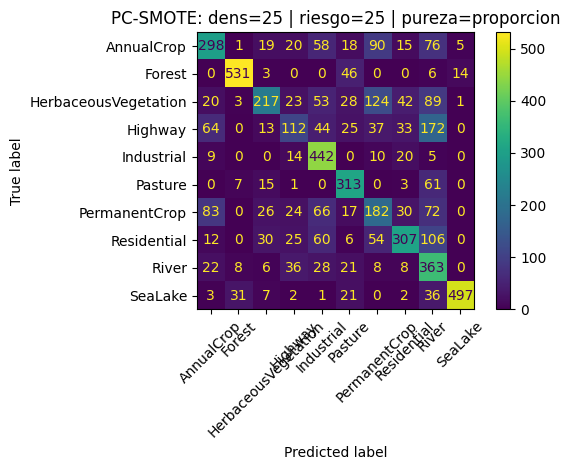
\includegraphics[width=0.6\textwidth]{pcsmote_heatmap_best.png}
  \caption{Matriz de confusión para la mejor configuración de PC-SMOTE (densidad=25, riesgo=25, pureza=proporción)}
  \label{fig:pcsmote_best_heatmap}
\end{figure}

\begin{figure}[H]
  \centering
  \includegraphics[width=0.6\textwidth]{proyeccion_3d_sinteticos.png}
  \caption{Visualización 3D del espacio generado por PC-SMOTE}
  \label{fig:proyeccion_3d_sinteticos}
\end{figure}

% Tablas comparativas, mejores configuraciones, mat. conf.
% Referencia a heatmap, e.g. “ver Figura X”

\section{Discusión}

Los resultados obtenidos permitieron identificar patrones relevantes en el comportamiento de las técnicas de sobremuestreo y su interacción con distintos clasificadores y datasets. En esta sección se analizan los hallazgos más significativos y se discuten sus implicancias.

\subsection{Desempeño de las técnicas avanzadas}

Las variantes más recientes como PC-SMOTE, AR-ADASYN y α‑DBASMOTE mostraron ventajas claras frente a los métodos tradicionales. Su capacidad para incorporar información estructural del espacio de características (como densidad, riesgo o pureza) contribuyó a una generación más eficiente de ejemplos sintéticos, minimizando el sobreajuste y reduciendo el ruido.

Se destacó la versión combinada α‑DBASMOTE + AR‑ADASYN por su robustez frente a diferentes tipos de desbalance, logrando un equilibrio entre diversidad y precisión. Esta técnica combinada aprovechó la identificación geométrica precisa de zonas frontera (α‑DBASMOTE) y una generación adaptativa focalizada en muestras peligrosas (AR-ADASYN).

\subsection{Importancia del clasificador elegido}

La elección del clasificador también influyó significativamente en los resultados. Modelos como XGBoost y Gradient Boosting mostraron una mayor capacidad para capturar estructuras complejas en los datos sintéticos, mientras que métodos como KNN fueron más sensibles a la calidad del sobremuestreo. Esto refuerza la idea de que la selección del clasificador no debe disociarse de la técnica de balanceo utilizada.

\subsection{Limitaciones observadas}

Algunas técnicas, como ADASYN y Borderline-SMOTE, presentaron limitaciones en datasets con bajo volumen de datos o fuerte solapamiento entre clases. En ciertos casos, la generación excesiva de ejemplos en zonas ruidosas incrementó la tasa de falsos positivos. Además, si bien PC-SMOTE ofreció un buen rendimiento general, su eficacia dependió de una cuidadosa calibración de parámetros.

Finalmente, se observó que los resultados variaron considerablemente entre datasets, lo que sugiere que no existe una técnica universalmente superior. Cada combinación de dataset, técnica de sobremuestreo y clasificador planteó desafíos específicos, lo que justifica la necesidad de realizar estudios comparativos como el presente.

\subsection{Implicancias}

Este análisis confirmó la relevancia de evaluar técnicas de sobremuestreo bajo un enfoque integral, considerando tanto su formalización teórica como su impacto práctico sobre el rendimiento de clasificación. Además, la inclusión de visualizaciones y métricas múltiples permitió una comprensión más profunda del efecto de cada técnica sobre la geometría del espacio de características.

% Interpretación de resultados, comparativas, limitaciones

\section{Conclusiones y trabajos futuros}

El presente trabajo tuvo como objetivo analizar, implementar y comparar distintas técnicas de sobremuestreo en contextos de clasificación con datos desbalanceados. Se evaluaron métodos tradicionales como SMOTE, ADASYN y Borderline-SMOTE, así como variantes recientes como PC-SMOTE, AR-ADASYN y α‑DBASMOTE, tanto en sus versiones individuales como combinadas.

Los resultados obtenidos confirmaron que las técnicas avanzadas, al incorporar criterios de densidad, riesgo y pureza, ofrecieron mejoras sustanciales en métricas como F1-score y AUC-ROC. En particular, la técnica híbrida α‑DBASMOTE + AR‑ADASYN logró un desempeño superior en varios escenarios, combinando una selección precisa de muestras críticas con una generación adaptativa de ejemplos sintéticos.

Además, se observó que el rendimiento final dependió no solo del método de sobremuestreo, sino también del clasificador utilizado y del dataset evaluado. Esta dependencia resalta la importancia de realizar evaluaciones integrales que contemplen múltiples combinaciones de técnicas y clasificadores.

Como trabajos futuros, se identificaron varias líneas de exploración:

\begin{itemize}
  \item Incorporar estrategias de selección de atributos para mejorar la calidad de las instancias generadas.
  \item Extender el análisis a datasets multietiqueta o secuenciales, donde el problema del desbalance presenta nuevas complejidades.
  \item Aplicar los algoritmos propuestos en dominios reales, como imágenes médicas o series temporales, evaluando su desempeño en entornos no controlados.
  \item Diseñar variantes más eficientes computacionalmente que mantengan la precisión sin aumentar el costo de entrenamiento.
\end{itemize}

En síntesis, esta investigación aportó evidencia empírica y formal sobre la eficacia de nuevas estrategias de sobremuestreo, destacando su potencial para mejorar la clasificación en dominios complejos y desbalanceados.

% Síntesis, aporte teórico-práctico, sugerencias


\section{Aportes esperados} 
\noindent\hyperlink{toc}{\small$\uparrow$ Volver al índice}

Desde una perspectiva académica, se espera que este trabajo constituya un aporte a la línea de investigación en preprocesamiento de datos y diseño de algoritmos orientados a escenarios de aprendizaje automático con clases desbalanceadas.

El principal aporte consiste en el desarrollo de una técnica híbrida que integra mecanismos de selección y generación sintética basados en fundamentos geométricos y adaptativos. En concreto, se propuso un modelo que combina técnicas de selección de instancias peligrosas con esquemas de generación de datos modernos. La hipótesis central fue que esta integración permitiría generar muestras sintéticas más representativas y útiles para el clasificador, especialmente en regiones de frontera donde las clases presentan solapamiento o alta variabilidad interna.

Como segundo aporte, se diseñó una nueva variante que extiende el enfoque clásico de SMOTE mediante la incorporación de criterios adaptativos en sus tres fases principales: (i) selección de muestras minoritarias, (ii) elección filtrada de vecinos representativos, y (iii) ajuste del parámetro de interpolación que determina la posición relativa de las muestras generadas. La hipótesis planteada fue que esta estrategia permitiría un control más preciso sobre la distribución de las muestras sintéticas, adecuándose mejor a la morfología del espacio de decisión y mitigando la generación de ruido o redundancia.

Ambas líneas de desarrollo buscan mejorar la capacidad de generalización de los clasificadores en contextos reales, tanto en clasificación binaria como multiclase, y servir como base para futuros trabajos que exploren la combinación de mecanismos estructurales con esquemas de generación controlada de datos sintéticos.

\section{Referencias bibliográficas} \noindent\hyperlink{toc}{\small$\uparrow$ Volver al índice}
\printbibliography

\appendix

\section{Código fuente del pipeline experimental}
\label{apendice:codigo_pipeline}

A continuación se presenta el código fuente del script en Python utilizado para la ejecución masiva de experimentos con técnicas de sobremuestreo:


\begin{lstlisting}[language=Python, caption={Script de experimentación automática}, label={lst:script_experimento}]
# 1. Importación de librerías necesarias
# Se importan todas las librerías necesarias para:
# - Manipular archivos (os)
# - Cargar y procesar datos (pandas, numpy)
# - Modelado y métricas (sklearn)
# - Técnicas de sobremuestreo (imblearn)
# - Visualización (seaborn, matplotlib)

import os
import pandas as pd
import numpy as np
from sklearn.model_selection import train_test_split
from sklearn.preprocessing import StandardScaler
from sklearn.ensemble import RandomForestClassifier
from sklearn.linear_model import LogisticRegression
from sklearn.neighbors import KNeighborsClassifier
from sklearn.metrics import classification_report, confusion_matrix
from imblearn.over_sampling import SMOTE, ADASYN, BorderlineSMOTE
import seaborn as sns
import matplotlib.pyplot as plt
from collections import Counter

# 2. Preparación de carpetas de salida
# Crear carpetas para guardar resultados gráficos (figures) y tabulares (resultados)
os.makedirs("../figures", exist_ok=True)
os.makedirs("../resultados", exist_ok=True)

# 3. Definición de modelos y técnicas de sobremuestreo
# Se combinan tres clasificadores con tres técnicas de balanceo
modelos = {
    "RandomForest": RandomForestClassifier(random_state=42),
    "LogisticRegression": LogisticRegression(max_iter=1000),
    "KNN": KNeighborsClassifier()
}

tecnicas = {
    "SMOTE": SMOTE(random_state=42),
    "ADASYN": ADASYN(random_state=42),
    "BorderlineSMOTE": BorderlineSMOTE(random_state=42)
}

# 4. Conversión de rangos tipo '1-9' al promedio (ej: '1-9' => 5.0)
def convertir_rango(valor):
    if isinstance(valor, str) and '-' in valor:
        try:
            inicio, fin = map(float, valor.split('-'))
            return (inicio + fin) / 2
        except:
            return np.nan
    return valor

# 5. Procesamiento principal por dataset
ruta_datasets = "../datasets"
datasets = [d for d in os.listdir(ruta_datasets) if os.path.isdir(os.path.join(ruta_datasets, d))]

for nombre_dataset in datasets:
    print(f"Procesando dataset: {nombre_dataset}")
    carpeta = os.path.join(ruta_datasets, nombre_dataset)
    archivos_data = [f for f in os.listdir(carpeta) if f.endswith(".data")]
    if not archivos_data:
        print(f"No se encontró archivo .data en {nombre_dataset}, se omite.")
        continue
    path_data = os.path.join(carpeta, archivos_data[0])

    # Carga robusta de archivos (con fallback a latin1 y separadores especiales)
    try:
        df = pd.read_csv(path_data, header=None, na_values='?')
        if df.shape[1] <= 1:
            df = pd.read_csv(path_data, header=None, na_values='?', sep='\s+')
        if df.iloc[0].apply(lambda x: isinstance(x, str) and not x.replace('.', '', 1).isdigit()).any():
            df = df.iloc[1:].reset_index(drop=True)
    except UnicodeDecodeError:
        try:
            df = pd.read_csv(path_data, header=None, na_values='?', encoding='latin1', sep='\s+', on_bad_lines='skip')
        except Exception as e2:
            print(f"Error cargando {nombre_dataset} con latin1: {e2}")
            continue
    except Exception as e:
        print(f"Error cargando {nombre_dataset}: {e}")
        continue

    try:
        # Limpieza de datos
        if df.dtypes[0] == 'object':
            df = df.drop(columns=df.columns[0])
        df = df.astype(str).apply(lambda col: col.map(convertir_rango))
        df.replace('?', np.nan, inplace=True)
        df = df.apply(pd.to_numeric, errors='coerce')
        df.dropna(inplace=True)

        X = df.iloc[:, :-1]
        y = df.iloc[:, -1]
        if len(np.unique(y)) < 2:
            print(f"Saltando {nombre_dataset} por tener una sola clase")
            continue

        # Escalado
        scaler = StandardScaler()
        X_scaled = scaler.fit_transform(X)

        resultados = []

        # Combinaciones modelo + técnica
        for nombre_modelo, modelo in modelos.items():
            for nombre_tecnica, sampler in tecnicas.items():
                X_res, y_res = sampler.fit_resample(X_scaled, y)

                min_clase = min(Counter(y_res).values())
                if "Borderline" in nombre_tecnica and min_clase < 6:
                    continue
                if "KNN" in nombre_modelo and min_clase < 6:
                    continue

                X_train, X_test, y_train, y_test = train_test_split(X_res, y_res, test_size=0.3, random_state=42)
                modelo.fit(X_train, y_train)
                y_pred = modelo.predict(X_test)

                # Reporte y visualización
                report = classification_report(y_test, y_pred, output_dict=True)
                cm = confusion_matrix(y_test, y_pred)
                plt.figure(figsize=(5, 4))
                sns.heatmap(cm, annot=True, fmt="d", cmap="Blues")
                plt.title(f"{nombre_dataset} - {nombre_modelo} + {nombre_tecnica}")
                plt.xlabel("Predicción")
                plt.ylabel("Real")
                plt.tight_layout()
                plt.savefig(f"../figures/{nombre_dataset}_{nombre_modelo}_{nombre_tecnica}_heatmap.png")
                plt.close()

                # Registro de resultados
                labels = list(map(str, sorted(np.unique(y))))
                entry = {
                    "Dataset": nombre_dataset,
                    "Modelo": nombre_modelo,
                    "Técnica": nombre_tecnica,
                    "Accuracy": report.get("accuracy", 0)
                }
                for label in labels:
                    if label in report:
                        entry[f"Precision ({label})"] = report[label]["precision"]
                        entry[f"Recall ({label})"] = report[label]["recall"]
                        entry[f"F1-score ({label})"] = report[label]["f1-score"]
                    else:
                        entry[f"Precision ({label})"] = None
                        entry[f"Recall ({label})"] = None
                        entry[f"F1-score ({label})"] = None
                resultados.append(entry)

        df_resultados = pd.DataFrame(resultados)
        df_resultados.to_csv(f"../resultados/resultados_{nombre_dataset}.csv", index=False)
        print(f"✓ Resultados guardados para {nombre_dataset}\n")

    except Exception as e:
        print(f"Error procesando {nombre_dataset}: {e}\n")
\end{lstlisting}




\end{document}
